\documentclass[a4paper,12pt]{article}
\usepackage{outline}
\usepackage{pmgraph}
\usepackage[normalem]{ulem}
\usepackage{comment} % enables the use of multi-line comments (\ifx \fi)
\usepackage{lipsum} %This package just generates Lorem Ipsum filler text.
\usepackage{fullpage} % changes the margin
\usepackage{listings}
\usepackage{color}
\usepackage{mdframed}
\usepackage{listings}
\usepackage{amssymb}
\usepackage{amsmath}
\usepackage{graphicx}
\usepackage{caption}
\usepackage{tikz}
\graphicspath{ {../} }
\renewcommand{\lstlistingname}{Code Block}% Listing -> Algorithm
\renewcommand{\lstlistlistingname}{List of \lstlistingname s}% List of Listings -> List of Algorithms

\linespread{1.5}
%--------------------Indention
\setlength{\parindent}{15pt}
\lstset{frame=shadowbox, rulesepcolor=\color{white}}
\mdfsetup{frametitlealignment=\center}
\lstset{
  numbers=left,
  stepnumber=1,
  firstnumber=1,
  numberfirstline=true
}

\begin{document}
\section*{Prelab}
\begin{enumerate}
  \item \textbf{Fill in the remaining entries in Table 1. You may find the discussion on Generating Timing Delays in the background section helpful.}
  
    \begin{center}
      \captionof{table}{Traffic Light Controller States}
      \begin{tabular}{|c||c|c|c|c|}
         \hline
         State & Highway Output & Farm Road Output & Delay (seconds) & Delay (cc) \\
         \hline
         \hline
         S0 & red & red & 1 & 50,000,000\\
         \hline
         S1 & green & red & 30 & 1,500,000,000\\
         \hline
         S2 & yellow & red & 3 & 150,000,000\\
         \hline
         S3 & red & red & 1 & 50,000,000\\
         \hline
         S4 & red & green & 15 & 750,000,000\\
         \hline
         S5 & red & yellow & 3 & 150,000,000\\
         \hline
      \end{tabular}
    \end{center}
  
  \item \textbf{Based on the column entries you just calculated, what is the necessary value of n in Figure 5?}
  
  The largest number that will need to be represented in binary is 1,500,000,000. That number in binary is 1011001011010000010111100000000 which consits of 31 bits thus $n=31$ wires.
  
  \item \textbf{Given Table 1 and Figure 6, create a state diagram for the traffic light controller FSM. Be sure to include the appropriate input and output labels. Assume S0 is the reset state.}
  
\begin{center}
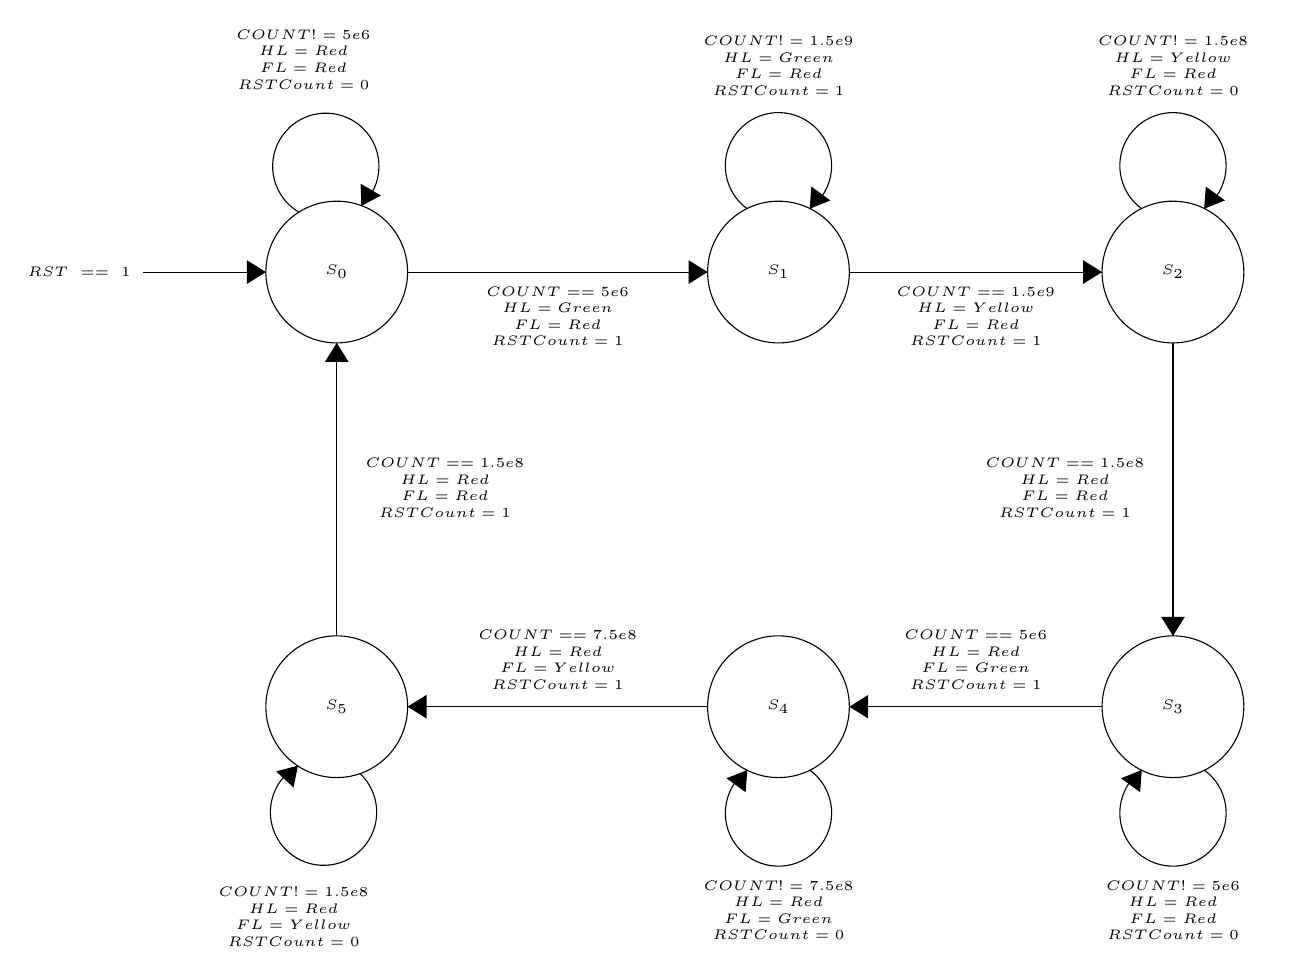
\begin{tikzpicture}[scale=0.3]
\tiny
\tikzstyle{every node}+=[inner sep=0pt]
\draw [black] (15.4,-19.4) circle (3);
\draw (15.4,-19.4) node {$S_0$};
\draw [black] (34.1,-19.4) circle (3);
\draw (34.1,-19.4) node {$S_1$};
\draw [black] (50.8,-19.4) circle (3);
\draw (50.8,-19.4) node {$S_2$};
\draw [black] (50.8,-37.8) circle (3);
\draw (50.8,-37.8) node {$S_3$};
\draw [black] (34.1,-37.8) circle (3);
\draw (34.1,-37.8) node {$S_4$};
\draw [black] (15.4,-37.8) circle (3);
\draw (15.4,-37.8) node {$S_5$};
\draw [black] (18.4,-19.4) -- (31.1,-19.4);
\fill [black] (31.1,-19.4) -- (30.3,-18.9) -- (30.3,-19.9);
\draw (24.75,-19.9) node [below] {\begin{tabular}{c} $COUNT == 5e6$ \\ $HL = Green$ \\ $FL = Red$ \\ $RSTCount = 1$ \end{tabular}};
\draw [black] (37.1,-19.4) -- (47.8,-19.4);
\fill [black] (47.8,-19.4) -- (47,-18.9) -- (47,-19.9);
\draw (42.45,-19.9) node [below] {\begin{tabular}{c} $COUNT == 1.5e9$ \\ $HL = Yellow$ \\ $FL = Red$ \\ $RSTCount = 1$ \end{tabular}};
\draw [black] (50.8,-22.4) -- (50.8,-34.8);
\fill [black] (50.8,-34.8) -- (51.3,-34) -- (50.3,-34);
\draw (50.3,-28.6) node [left] {\begin{tabular}{c} $COUNT == 1.5e8$ \\ $HL = Red$ \\ $FL = Red$ \\ $RSTCount = 1$ \end{tabular}};
\draw [black] (47.8,-37.8) -- (37.1,-37.8);
\fill [black] (37.1,-37.8) -- (37.9,-38.3) -- (37.9,-37.3);
\draw (42.45,-37.3) node [above] {\begin{tabular}{c} $COUNT == 5e6$ \\ $HL = Red$ \\ $FL = Green$ \\ $RSTCount = 1$ \end{tabular}};
\draw [black] (31.1,-37.8) -- (18.4,-37.8);
\fill [black] (18.4,-37.8) -- (19.2,-38.3) -- (19.2,-37.3);
\draw (24.75,-37.3) node [above] {\begin{tabular}{c} $COUNT == 7.5e8$ \\ $HL = Red$ \\ $FL = Yellow$ \\ $RSTCount = 1$ \end{tabular}};
\draw [black] (16.38,-40.623) arc (46.87498:-241.12502:2.25);
\draw (13.57,-45.32) node [below] {\begin{tabular}{c} $COUNT != 1.5e8$ \\ $HL = Red$ \\ $FL = Yellow$ \\ $RSTCount = 0$ \end{tabular}};
\fill [black] (13.76,-40.29) -- (12.84,-40.54) -- (13.57,-41.22);
\draw [black] (35.423,-40.48) arc (54:-234:2.25);
\draw (34.1,-45.05) node [below] {\begin{tabular}{c} $COUNT != 7.5e8$ \\ $HL = Red$ \\ $FL = Green$ \\ $RSTCount = 0$ \end{tabular}};
\fill [black] (32.78,-40.48) -- (31.9,-40.83) -- (32.71,-41.42);
\draw [black] (52.123,-40.48) arc (54:-234:2.25);
\draw (50.8,-45.05) node [below] {\begin{tabular}{c} $COUNT != 5e6$ \\ $HL = Red$ \\ $FL = Red$ \\ $RSTCount = 0$ \end{tabular}};
\fill [black] (49.48,-40.48) -- (48.6,-40.83) -- (49.41,-41.42);
\draw [black] (49.477,-16.72) arc (234:-54:2.25);
\draw (50.8,-12.15) node [above] {\begin{tabular}{c} $COUNT != 1.5e8$ \\ $HL = Yellow$ \\ $FL = Red$ \\ $RSTCount = 0$ \end{tabular}};
\fill [black] (52.12,-16.72) -- (53,-16.37) -- (52.19,-15.78);
\draw [black] (32.777,-16.72) arc (234:-54:2.25);
\draw (34.1,-12.15) node [above] {\begin{tabular}{c} $COUNT != 1.5e9$ \\ $HL = Green$ \\ $FL = Red$ \\ $RSTCount = 1$ \end{tabular}};
\fill [black] (35.42,-16.72) -- (36.3,-16.37) -- (35.49,-15.78);
\draw [black] (13.809,-16.871) arc (239.90614:-48.09386:2.25);
\draw (13.99,-11.89) node [above] {\begin{tabular}{c} $COUNT != 5e6$ \\ $HL = Red$ \\ $FL = Red$ \\ $RSTCount = 0$ \end{tabular}};
\fill [black] (16.44,-16.6) -- (17.27,-16.16) -- (16.41,-15.66);
\draw [black] (15.4,-34.8) -- (15.4,-22.4);
\fill [black] (15.4,-22.4) -- (14.9,-23.2) -- (15.9,-23.2);
\draw (15.9,-28.6) node [right] {\begin{tabular}{c} $COUNT == 1.5e8$ \\ $HL = Red$ \\ $FL = Red$ \\ $RSTCount = 1$ \end{tabular}};
\draw [black] (7.2,-19.4) -- (12.4,-19.4);
\draw (6.7,-19.4) node [left] {$RST\mbox{ }==\mbox{ }1$};
\fill [black] (12.4,-19.4) -- (11.6,-18.9) -- (11.6,-19.9);
\end{tikzpicture}
\end{center}

  
  \item \textbf{Now describe the traffic light controller FSM in Verilog using the following module interface}
  
  % Verilog code template
\lstinputlisting[language=Verilog,,caption=TLC FSM Verilog ]{tlc_fsm.v}
\end{enumerate}



\ifx
\section*{Design}

% Verilog code template
% \lstinputlisting[language=Verilog,,caption=4-Bit ALU ]{../code name.v}

\section*{Results}

% Figure with caption
% \begin{figure}[h]
%   \begin{center}
%     \includegraphics[scale=1]{2_1MuxPlot.png}
%     \caption{\textit{2-Bit 2:1 MUX Plots}}
%   \end{center}
% \end{figure}


\section*{Conclusion}


\section*{Questions}

\begin{enumerate}
  \item 1.
\end{enumerate}

\section*{Student Feedback}

\begin{enumerate}
  \item \textbf{What did you like most about the lab assignment and why? What did you like least about it and why?}
  \vspace{10pt}

  \item \textbf{Were there any section of the lab manual that were unclear? If so, what was unclear? Do you have any suggestions for improving the clarity?}
  \vspace{10pt}

  \item \textbf{What suggestions do you have to improve the overall lab assignment?}
  \vspace{10pt}

\end{enumerate}


\begin{thebibliography}{1}
\bibitem{Verilog} Charles Kime \& Thomas Kaminski  \emph{Logic and Computer Design Fundamentals} \\ \hspace{15pt}\textit{http://www.cs.bilkent.edu.tr/~will/courses/CS223/Verilog/LCDF3_Verilog_Ch_4.pdf}
\end{thebibliography}

\section*{Attachments}
%Make sure to change these
Lab Notes, HelloWorld.ic, FooBar.ic
%\fi %comment me out

\begin{thebibliography}{9}
\bibitem{Verilog} Charles Kime & Thomas Kaminski  \emph{Logic and Computer Design Fundamentals} \textit{http://www.cs.bilkent.edu.tr/~will/courses/CS223/Verilog/LCDF3_Verilog_Ch_4.pdf}
\end{thebibliography}

%How to cite
Put your Problem statement here! Example of a Citation\cite[p.219]{Robotics}. Here's Another Citation\cite{Flueck}
\fi
\end{document}
